\documentclass[a4paper,12pt]{article}

\usepackage[14pt]{extsizes}
\usepackage{cmap}					% поиск в PDF
\usepackage{mathtext} 				% русские буквы в фомулах
\usepackage[T2A]{fontenc}			% кодировка
\usepackage[utf8]{inputenc}			% кодировка исходного текста
\usepackage[english,russian]{babel}	% локализация и переносы
\usepackage{graphicx}
\usepackage{geometry}
\usepackage{amsmath}
\usepackage[table]{xcolor}

\geometry{verbose, a4paper, tmargin=2cm, bmargin=2cm, lmargin=3cm, rmargin=2cm}
\author{Vysotsky Maxim}
\title{Отчёт}
\date{2022}

\begin{document}
\begin{titlepage}
	\begin{center}
		{Министерство науки и высшего образования Российской Федерации
			НАЦИОНАЛЬНЫЙ ИССЛЕДОВАТЕЛЬСКИЙ ТОМСКИЙ
			ГОСУДАРСТВЕННЫЙ УНИВЕРСИТЕТ (НИ ТГУ)}
	\end{center}
	\begin{center}
		{Физический факультет}
	\end{center}
	
	
	\vspace{8cm}
	{
		\begin{center}
			{\bf Лабораторная работа на тему}\\
			Определение коэффициента внутреннего трения газа
			капиллярным вискозиметром
		\end{center}
	}
	\vspace{2cm}
	\begin{flushright}
		{Руководитель:\\ канд. физ.-мат. наук\\
			И. А. Конов\\
			Работу выполнили:\\
			Н. Н. Левин\\
			М. Ю. Высоцкий\\
			\vspace{0.2cm}
			гр. 052101}
	\end{flushright}
	\vspace{3cm}
	\begin{center}
		Томск, 2022
	\end{center}
\end{titlepage}

\section{Теоретическое введение}
\textbf{Цель работы:} определение коэффициента вязкости воздуха при
комнатной температуре. Вычисление средней длины свободного
пробега молекул воздуха.

\subsection{Вязкость}
В равновесном состоянии различные части фазы покоятся друг относительно друга. При их относительном движении возникают силы торможения (вязкость), которые стремятся снизить относительную скорость. Механизм возникновения внутреннего трения между слоями газа заключается в обмене молекул между ними (в силу хаотичного тепловогодвижения). Таким образом, импульс более быстрого слоя уменьшается, а
медленного - увеличивается. Данный процесс можно рассматривать как
передачу импульса за единицу времени от слоя к слою, что по второму
закону Ньютона дают нам силу, направленную по касательной к поверх-
ности слоёв. Величина данной силы была установлена Ньютоном, и был
ввыведен закон:

\begin{equation}\label{newton}
F = \eta\frac{dU}{dx}S,
\vspace{0.3cm}
\end{equation}
где $\frac{dU}{dx}$ - градиент скорости, $\eta$ - \textbf{коэффициент вязкости}.

\begin{figure}[h!]
\begin{center}
	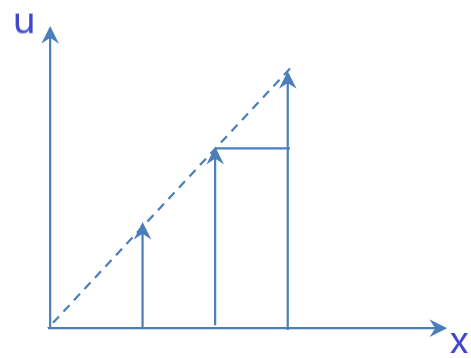
\includegraphics[scale=0.3]{1}
\end{center}
\caption{зависимость u(x)}
\end{figure}


Из формулы \eqref{newton} следует, что размерность коэффициента вязкости - Паскаль-секунда.
Физический смысл коэффициента вязкости выявляется при рассмот
рении хаотического движения молекул газа, переносящих импульс упорядоченного движения $mU$.

На рисунке 1 показаны векторы скоростей слоёв, перпендикулярных оси $x$. Произвольно выбранный слой движется медленнее, чем слой, расположенный справа, и быстрее, чем слой, расположенный слева. Разбиение на слои сделано условно, $\Delta x$ - расстояние между слоями, скорости которых отличаются на $\Delta U$. Из-за теплового движения молекулы перемещаются из слоя в слой, притом каждая частица переносит свой импульс $mU$.

Сила трения $\tau$, отнесенная к площади соприкасающихся повехностей газа, равна плотности потока импульса $G_{mU}$ упорядоченного движения, переносимого молекулами в перпендикулярном скорости направлении.

В идеальном газе для плотности $G_{mU}$ получено выражение:
\begin{equation}
G_{mU} = -\frac{1}{3}n_0<v><l>m\frac{\partial U}{\partial x},
\end{equation}
где $n_0$ - концентрация газа, $<v>$ - средняя скорость хаотичного движения молекул, $m$ - масса молекулы, $<l>$ - средняя длина свободного пробега.

Таким образом, 
\begin{equation}\label{tau}
\tau = -\eta\frac{\partial U}{\partial x} = -\frac{1}{3}n_0<v><l>m\frac{\partial U}{\partial x}
\end{equation}

Знак $\tau$ указывает, что сила трения направлена \textbf{против скорости}.

Как следует из \eqref{tau}, динамическая вязкость может быть представлена в виде:
\begin{equation}\label{tau}
\eta = \frac{1}{3}n_0<v><l>m = \frac{1}{3}\rho<v><l>
\end{equation}

Динамическая вязкость не зависит от давления и растет в основном пропорционально квадратному корню от температуры.

\newpage
\subsection{Протекание газа через капилляр. Формула Пуазейля}
Рассмотрим движение в трубке. Она изображена на рисунке 2. Движение газа будем считать \textbf{ламинарным}. Выделим внутри трубки два коаксиальных цилиндра: первый - радиуса $r$, а второй - радиуса $R$.

\begin{figure}[h!]
	\begin{center}
		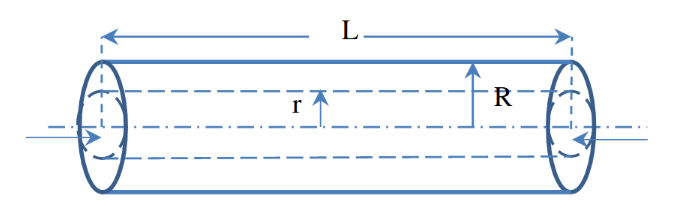
\includegraphics[scale=0.7]{2}
	\end{center}
	\caption{зависимость u(x)}
\end{figure}

При ламинарном (стационарном) течении сумма всех сил, действующих на поверхность выделенного объема, будет равна нулю. Следовательно:
$$P_1\pi r^2 - P_2\pi r^2 - F_{тр}= 0,$$
где $P_1\pi r^2$, $P_2\pi r^2$ -- силы давления на торцы цилиндра, $F_{тр}$ -- сила внутреннего трения, действующая по боковой поверхности цилиндра.
$$F_{тр} = \tau S,$$
где $S = 2\pi rL$ -- площадь боковой поверхности цилиндра и, согласно уравнению \eqref{tau},
$$\tau = -\eta\frac{\partial U}{\partial r}$$
Таким образом, получаем дифференциальное уравнение:
$$\pi r^2P_1 - P_2 + \eta2\pi rL\frac{dU}{dr} = 0,$$
которое решается методом разделение переменных и интегрированием. После чего находится постоянная интегрирования:
$$dU = -\frac{P_1 - P_2}{2L\eta}rdr$$
$$U = -\frac{P_1 - P_2}{4L\eta}r^2 + C$$
При r = R скорость равна нулю, следовательно:

$$C = \frac{P_1 - P_2}{4L\eta}R^2$$
В результате имеем закон распределения скоростей по сечению трубы:
\begin{equation}\label{distrib}
U = \frac{P_1 - P_2}{4L\eta}(R^2-r^2)
\end{equation}
Найдем зависимость между расходом газа и разностью давлений на
концах капилляра. \textbf{Расходом газа} Q называется объем газа, протекающий в единицу времени через поперечное сечение трубы.
Выделим кольцевую площадку с внутренним радиусом $r$ и внешним $r + dr (dS = 2\pi rdr)$. Тогда:
$$dQ = UdS = U2\pi rdr$$
$$Q = \frac{\Delta V}{\Delta t} = \pi\frac{P_1 - P_2}{2L\eta}(R^2-r^2)\bigg|_0^R \vspace{0.2cm}$$
После интегрирования:
\begin{equation}\label{pu}
Q = \pi\frac{P_1 - P_2}{8L\eta}R^4
\end{equation}

Полученное выражение \eqref{pu} носит название \textbf{формулы Пуазейля}. На применении данной формулы основан один из экспериментальных методов определения коэффициента вязкости:
\begin{equation}
\eta = \pi\frac{(P_1-P_2)\Delta t}{8L\Delta V}R^4
\end{equation}

\newpage
\section{Ход эксперимента}

\begin{center}
	\begin{tabular}{|c|c|c|c|c|}
		\hline

		№&dP, 1 мм в.с.&dt, c&dV, $\frac{м^3}{с}*10^{-5}$&$(\eta +\Delta\eta), \frac{Па}{с}$\\
		\hline
		1& 106 & 3,49 & 0,5 & 0,000088 ± 0,000008
		\\
		2& 110 & 4,37 & 0,5 & 0,000115 ± 0,000005
		\\
		3& 106 & 4,04 & 0,5 & 0,0001151 ± 0,0000013
		\\
		4& 106 & 3,87 & 0,5 & 0,000098 ± 0,000003
		\\
		5& 104 & 4,42 & 0,5 & 0,000110 ± 0,000002
		\\ 
		6& 108 & 4,54 & 0,5 & 0,000117 ± 0,000006
		\\
		\hline
	\end{tabular}
\end{center}

\end{document}